\documentclass[10pt]{article}
\usepackage{amsmath,textcomp,amssymb,geometry,graphicx,enumerate,tikz,algorithm,algpseudocode,pifont}
\usetikzlibrary{calc}
\usetikzlibrary{datavisualization}
\usetikzlibrary{datavisualization.formats.functions}


\textheight=9in
\textwidth=7in
\topmargin=-.75in
\oddsidemargin=-0.25in
\evensidemargin=-0.25in

\usepackage{listings}
\lstnewenvironment{codeblock}
    {\lstset{language=Python,
      showspaces=false,
      showtabs=false,
      breaklines=true,
      mathescape=true,
      showstringspaces=false,
      breakatwhitespace=true,
      commentstyle=\textit,
      keywordstyle=\textbf,
      basicstyle=\ttfamily,
      escapechar=`,
      moredelim={**[is][{\color{RoyalBlue}}]{\^^M\\beginsol}{\^^M\\endsol}},
      moredelim={[is][{\color{RoyalBlue}}]{\^^M\\beginexp}{\^^M\\endexp}},
    }}
    {}
    
\begin{document}
	\section*{02/24/2016}
	\subsection*{Regression} aka fitting curves to data
	\begin{itemize}
		\item Classification: given sample $x$, predict class (often binary).
		\item Regression given sample, $x$, predict a numerical value.
		\begin{itemize}
			\item Choose form of regression function $h(x;p)$ with parameters $p$.
			\begin{itemize}
				\item like predictor function in classification.
			\end{itemize}
			\item Choose a cost function (objective function) to optimize.
			\begin{itemize}
				\item Usually based on a loss function; e.g. risk function = expected loss.
			\end{itemize}
		\end{itemize}
		\item Some regression functions:
			\begin{enumerate}
				\item Linear: $h(x; w, \alpha) = w^{T}x + \alpha$.
				\item Polynomial.
				\item Logistic: $h(x; w, \alpha) = s(w^{T}x + \alpha)$. Recall: logistic function $s(\gamma) = \frac{1}{1 + e^{-\gamma}}$
			\end{enumerate}
		\item Some loss functions: let $z$ be prediction $h(x)$; $y$ be true value.
			\begin{enumerate}
				\item[A.] $L(z, y) = (z-y)^{2}$ \underline{squared error}.
				\item[B.] $L(z, y) = |z-y|$ \underline{absolute error}.
				\item[C.] $L(z, y) = -yln(z)-(1-y)ln(1-z)$ \underline{logistic loss}.
			\end{enumerate}
		\item Some cost functions to minimize:
			\begin{enumerate}
				\item[a.] $J(h) = \frac{1}{n}sum_{i=1}^{n}L(h(X_{i}),y_{i})$ \underline{mean loss}.
				\item[b.] $J(h) = \max_{i=1}^{n} L(h(X_{i}, y_{i}))$ \underline{maximum loss}.
				\item[c.] $J(h) = \sum \omega_{i}L(h(X_{i}, y_{i}))$ \underline{weighted sum}.
				\item[d.] $J(h) = \frac{1}{n}\sum L(h(X_{i}, y_{i})) + \lambda|w|^{2}$ \underline{$\ell_{2}$ penalized/regularized}.
				\item[e.] $J(h) = \frac{1}{n}\sum L(h(X_{i}, y_{i})) + \lambda|w|$ \underline{$\ell_{1}$ penalized/regularized}.
			\end{enumerate}
			\item Some combinations:
			\
			\begin{center}
				\begin{tabular}{|c|c|c|c|c|}
					\hline
					Name & Regression & Loss & Cost & Algorithm\\
					\hline
					Least-squares linear regression & 1 & A & a & quadratic, minimize w/calculus\\
					Weighted least-squares linear & 1 & A & c & quadratic, minimize w/calculus\\
					Ridge regression & 1 & A & d & quadratic, minimize w/calculus\\
					Lasso & 1 & A & d & minimize w/gradient descent\\
					Logistic regression & 3 & C & a & minimize w/gradient descent\\
					Least absolute deviations & 1 & B & a & minimize w/linear program\\
					Chebyshev criterion & 1 & B & b & minimize w/linear program\\
					\hline
				\end{tabular}
			\end{center}
	\end{itemize}
	
	\subsection*{Least-Squares Linear Regression} 1 + A + a.
	\begin{itemize}
		\item Optimization problem:
			\begin{center}
				\begin{tabular}{|c|}
					\hline
					Find $w, \alpha$ that minimizes
					$\sum_{i=1}^{n} (x_{i}\cdot w + \alpha - y_{i})^{2}$\\
					\hline
				\end{tabular}\\
				[1em]
				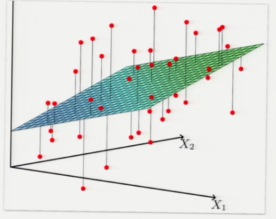
\includegraphics[scale=0.5]{../images/leastsquares}
			\end{center}
		\item Convention:
			\begin{itemize}
				\item $X$ is $n$x$d$ \underline{design matrix} of samples.
				\item $y$ is $d$-vector of dependent scalars.
				\item $X = \begin{bmatrix}
					x_{11} & x_{12} & \dots & x_{1d}\\
					x_{21} & x_{22} & \dots & \\
					\vdots & \vdots & \hdots & \\
					x_{n1} & x_{n2} & \dots & x_{nd}\\
				\end{bmatrix}$
				\item Usually $n > d$.
				\item Sample row vector is $X_{i}^{T}$.
				\item Column vector is $X_{*j}$.
				\item $y = \begin{bmatrix}
						y_{0}\\
						y_{1}\\
						\vdots\\
						y_{n}
				\end{bmatrix}$
				\item Recall fictitious dimension trick: replace $x\cdot w + \alpha$ with,
					\begin{align*}
						[x_{1} \ x_{2} \ \dots \ x_{d} \ 1] \cdot \begin{bmatrix}
								w_{1}\\
								w_{2}\\
								\vdots\\
								w_{d}\\
								\alpha
							\end{bmatrix}
					\end{align*}
					Now $X$ is an $n$x($d+1$) matrix; $w$ is a ($d+1$)-vector.
				\end{itemize}
			
			\item Rewritten optimization problem:
				\begin{center}
					\begin{tabular}{|c|}
						\hline
						Find $w$ that minimizes $|Xw-y|^{2}$\\
						\hline
					\end{tabular}\\
				\end{center}
			\item Optimize by calculus, minimize residual sum of squares:
				\begin{align*}
					RSS(w) &= w^{T}X^{T}Xw - 2y^{T}Xw + y^{T}y = 0\\
						&\implies X^{T}Xw = X^{T}y \Leftarrow \text{The \underline{normal equations}}
				\end{align*}
			\item If $X^{T}X$ is singular, problem is under-constrained.
			\item We use a linear solver to find $w = (X^{T}X)^{-1}X^{T}y$.
			\item $X^{+} = (X^{T}X)^{-1}X^{T}$ is the \underline{pseudoinverse} of $X$ and is a $(d+1)$x$n$ matrix.
			\item Observe: $X^{+}X = (X^{T}X)^{-1}X^{T}X = I \Leftarrow (d+1)\text{x}(d+1)$.
			\item Observe: the predicted values of $y$ are $\hat{y} = h(x;) \Rightarrow = Xw = XX^{+}y = Hy$.
			\item where $H = XX^{+}$ is the \underline{hat matrix} because it puts the hat on $y$.
			\item Interpretation as a projection:
				\begin{itemize}
					\item $\hat{y} = Xw \in \mathbb{R}^{n}$ is a linear combination of columns of $X$.
					\item For fixed $X$, varying $w$, $Xw$ is a subspace of $\mathbb{R}^{n}$ spanned by columns.
						\begin{center}
							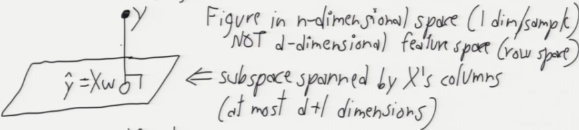
\includegraphics[scale=0.5]{../images/yhat}
						\end{center}
					\item Minimizing $|\hat{y} - y|$ find point $\hat{y}$ nearest $y$ on subspace $\Rightarrow$ project $y$ onto subspace.
					\item Error is smallest when line is perpendicular to subspace: $X^{T}(Xw-y) = 0 \Rightarrow$ the normal equations!
					\item Hat matrix $H$ (also called projection matrix) does the projecting. 
				\end{itemize}
			\item Advantages:
				\begin{itemize}
					\item Easy to compute; just solve a linear system.
					\item Unique, stable solution.
				\end{itemize}
			\item Disadvantages:
				\begin{itemize}
					\item Very sensitive to outliers, because error is squared!
					\item Fails if $X^{T}X$ is singular.
				\end{itemize}
	\end{itemize}
	
	\subsection*{Logistic Regression} (David Cox, 1953) 3 + C + a
		\begin{itemize}
			\item Fits "probabilities" in range (0, 1).
			\item Usually used for classification. The input $y_{i}$'s can be probabilities, but in most applications they are all 0 or 1.
			\item QDA, LDA: generative models.
			\item Logistic regression: discriminative model.
			\item Optimization problem:
				\begin{center}
					\begin{tabular}{|c|}
					\hline
						Find $w, \alpha$ that minimizes $J = \sum_{i=1}^{n}(y_{i} \ln s(X_{i} \cdot w + \alpha) + (1-y_{i}) \ln (1 - s(X_{i} \cdot w + \alpha))$\\
						\hline
					\end{tabular}\\
					[1em]
					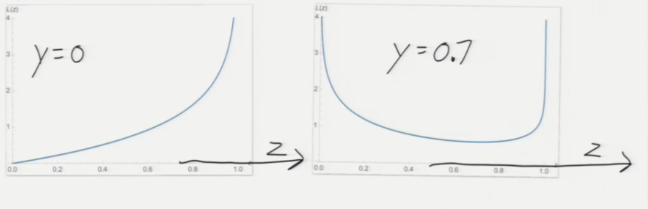
\includegraphics[scale=0.5]{../images/logistics}
				\end{center}
			\item $-J(w, \alpha)$ is convex. Solve by gradient ascent.
			\begin{align*}
				s'(\gamma) &= \frac{d}{d\gamma} \frac{1}{1 + e^{-\gamma}} = \frac{e^{-\gamma}}{(1 + e^{-\gamma})^{2}}\\
				&= s(\gamma)(1 - s(\gamma))\\
			\end{align*}
			\begin{center}
				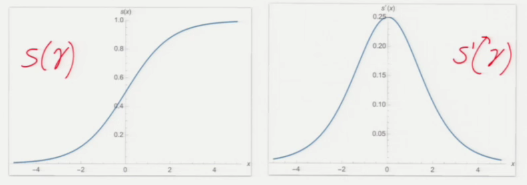
\includegraphics[scale=0.5]{../images/gradients}
			\end{center}
			\item Let $s_{i} = s(X_{i}\cdot w + \alpha)$,
			\begin{align*}
				\nabla_{w} J &= \sum\Big(\frac{y_{i}}{s_{i}}\nabla s_{i} - \frac{1-y_{i}}{1 - s_{i}} \nabla s_{i}\Big)\\
					&= \sum \Big(\frac{y_{i}}{s_{i}} - \frac{1-y_{i}}{1 - s_{i}}\Big) s_{i} (1 - s_{i})X_{i}\\
					&= \sum (y_{i} - s_{i})X_{i}
			\end{align*}
			
			\item Gradient ascent rule: $w \leftarrow w + \epsilon \sum_{i=1}^{n}(y_{i} - s(X_{i}\cdot w + \alpha))X_{i}$
			\item Stochastic gradient ascent: $w \leftarrow w + \epsilon(y_{i} - s(X_{i}\cdot w + \alpha))X_{i}$ works best if we shuffle samples in random order; process one by one.
			\item For very large $n$, sometimes converges before we visit all samples!
			\item Starting from $w=0, \alpha=0$ works well in practice.
			\begin{center}
				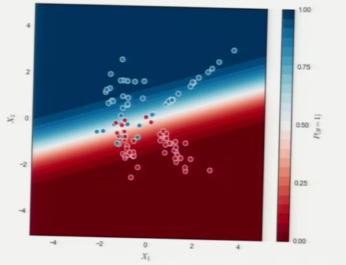
\includegraphics[scale=0.5]{../images/regression}
			\end{center}
		\end{itemize}
\end{document}